\documentclass[10pt]{article}
\usepackage[ngerman]{babel}
\usepackage[utf8]{inputenc}
\usepackage[T1]{fontenc}
\usepackage{graphicx}
\usepackage[export]{adjustbox}
\graphicspath{ {./images/} }
\usepackage{hyperref}
\hypersetup{colorlinks=true, linkcolor=blue, filecolor=magenta, urlcolor=cyan,}
\urlstyle{same}
\usepackage{amsmath}
\usepackage{amsfonts}
\usepackage{amssymb}
\usepackage[version=4]{mhchem}
\usepackage{stmaryrd}

\title{Bachelor of Science (BSc) in Informatik Modul Software-Entwicklung 1 (SWEN1) }

\author{}
\date{}


\begin{document}
\maketitle
\section*{LE 14 - Wrap-up der Vorlesung}
SWEN1/PM3 Team:\\
R. Ferri (feit), D. Liebhart (lieh), K. Bleisch (bles), G. Wyder (wydg)

\section*{Um was geht es?}
\begin{itemize}
  \item Was sind die wichtigen Themen und Schwerpunkte der Vorlesung?
  \item Wieviel weiss ich noch davon?
  \item Was ist genau der Inhalt der Semesterendprüfung?\\

\includegraphics[width=\linewidth]{images/2025_01_02_6eafa38dd4ae10c9a392g-02}
  \item Was muss ich allenfalls nochmals Repetieren für die Semesterendprüfung?
\end{itemize}

\section*{Lernziele LE 14 - Wrap up der Vorlesung}
\begin{itemize}
  \item Sie sind in der Lage:
  \item die wichtigsten Themen in der Vorlesung im Kontext eines iterativen Softwareentwicklungsprozesses kurz in eigenen Worten zu erläutern (Zweck, Prozesse und Artefakte).
  \item den Ablauf, Inhalt und die Prüfungsmodalitäten der Semesterendprüfung (SEP) zu erklären.
  \item besser einschätzen zu können, was Sie für die SEP noch repetieren müssen.
\end{itemize}

\begin{enumerate}
  \item Überblick
  \item Recap Anforderungsanalyse und
\end{enumerate}

Domänenmodellierung\\
3. Recap Softwarearchitektur und Design\\
4. Recap Entwurf mit Design Patterns\\
5. Info zur Semesterendprüfung\\
6. Bearbeitung einer Fallstudie (alte SEP)\\
7. Wrap-up

\begin{itemize}
  \item Sie sind in der Lage:
  \item für einen vorgegebenen, iterativ-inkrementellen Softwareentwicklungsprozess den Ablauf und die Artefakte zur Entwicklung einer objektorientierten Softwareapplikation zu erläutern,
  \item die Begriffswelt des Anwenders durch geeignete Vorgehensweisen erfassen und zu einer fachlichen Terminologie zu verdichten (Domänenmodell),
  \item eine Softwareapplikation sinnvoll abzugrenzen,
  \item systematisch die funktionalen Anforderungen mit Use Cases sowie Qualitätsanforderungen und Randbedingungen zu erheben und zu kommunizieren,
  \item basierend auf den Anforderungen eine geeignete Softwarearchitektur und ein objektorientiertes Design - Klassen mit Verantwortlichkeiten - für die darin enthaltenen Komponenten der fachlichen Logik zu entwerfen,
  \item für die Modellierung und Kommunikation von Artefakten im Softwareentwicklungsprozess standardisierte Notationen (wie UML) zu benutzen,
  \item bewährte Analyse, Architektur und Design Patterns adäquat für eine Problemstellung einzusetzen.
\end{itemize}

\section*{Themen und Ablauf des Moduls SWEN1}
School of

\begin{center}
\begin{tabular}{|c|l|}
\hline
SW\# & Thema \\
\hline
01 & Einführung und Überblick \\
\hline
02 & Anforderungsanalyse I \\
\hline
03 & Anforderungsanalyse II \\
\hline
04 & Domänenmodellierung \\
\hline
05 & \begin{tabular}{l}
Quizzy 1: Analyse \\
Softwarearchitektur und Design I \\
\hline
06 \\
\hline
\end{tabular} \\
\hline
07 & Softwarearchitektur und Design II \\
\hline
08 & Entwurf mit Design Patterns I \\
\hline
09 & Entwurf mit Design Patterns II \\
\hline
10 & Refactoring und Testing \\
\hline
11 & \begin{tabular}{l}
Quizzy 2: Design \\
Vertiefung 1: Verteilte Systeme \\
\hline
12 \\
\hline
\end{tabular} \\
\hline
13 & Vertiefung 2: Persistenz \\
\hline
14 & Vertiefung 3: Framework Design \\
\hline
\end{tabular}
\end{center}

\section*{Angewendeter iterativ-inkrementeller Softwareentwicklungsprozess in SWEN1/PM3}
\begin{itemize}
  \item Der Softwareentwicklungsprozess wurde so angepasst (engl. tailoring), dass die wesentlichen Artefakte in einem Softwareprojekt im Kontext eingeführt werden können.
  \item Die Software wird in Iterationen entwickelt (2 Wochen Rhythmus).
  \item Jede Iteration hat ein Ziel und wird nach Abschluss reviewed.
  \item Es gibt drei Meilensteine, die im Projektverlauf ein besonderes Ereignis darstellen bzw. den Abschluss einer Phase: Projektskizze (M1), Lösungsarchitektur (M2) und Beta-Release (M3)
  \item In jeder Iteration werden Anforderungen, Analyse \& Design, Implementation und Testing gemacht (Software entsteht in Inkrementen).
  \item Der angewendete Softwareentwicklungsprozess und das Projektmanagement eines iterativ-inkrementellen Projektes wird in PM3 noch detaillierter erklärt.
\end{itemize}

\section*{Wesentliche Resultate bzw. Artefakte}
\begin{itemize}
  \item Anforderungsanalyse
  \item Funktionale Anforderungen mit Use Cases
  \item Qualitätsanforderungen und Randbedingungen
  \item Domänenmodell
  \item Design
  \item Softwarearchitektur
  \item Use Case Realisierung (statische und dynamische Modelle)
  \item Implementation
  \item Quellcode (inkl. Javadoc)
  \item Testing
  \item Unit-Tests\\
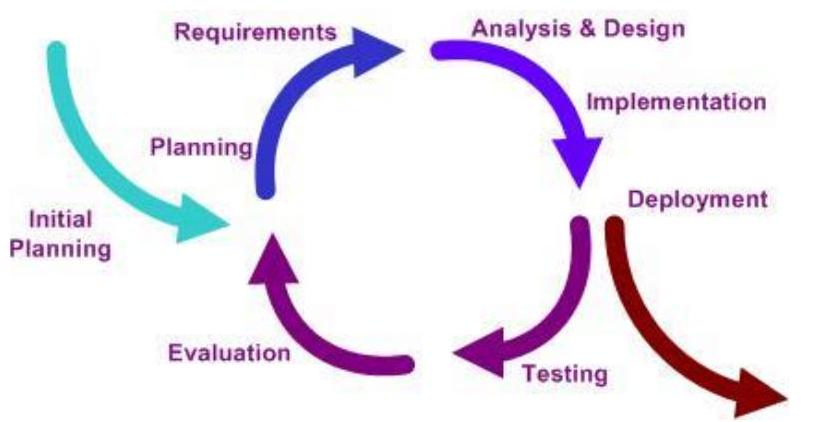
\includegraphics[width=\linewidth]{images/2025_01_02_6eafa38dd4ae10c9a392g-09}
  \item Integrations- und Systemtests
\end{itemize}

\section*{Modellierung und Modelle mit der UML}

\includegraphics[width=\linewidth]{images/2025_01_02_6eafa38dd4ae10c9a392g-10}\\
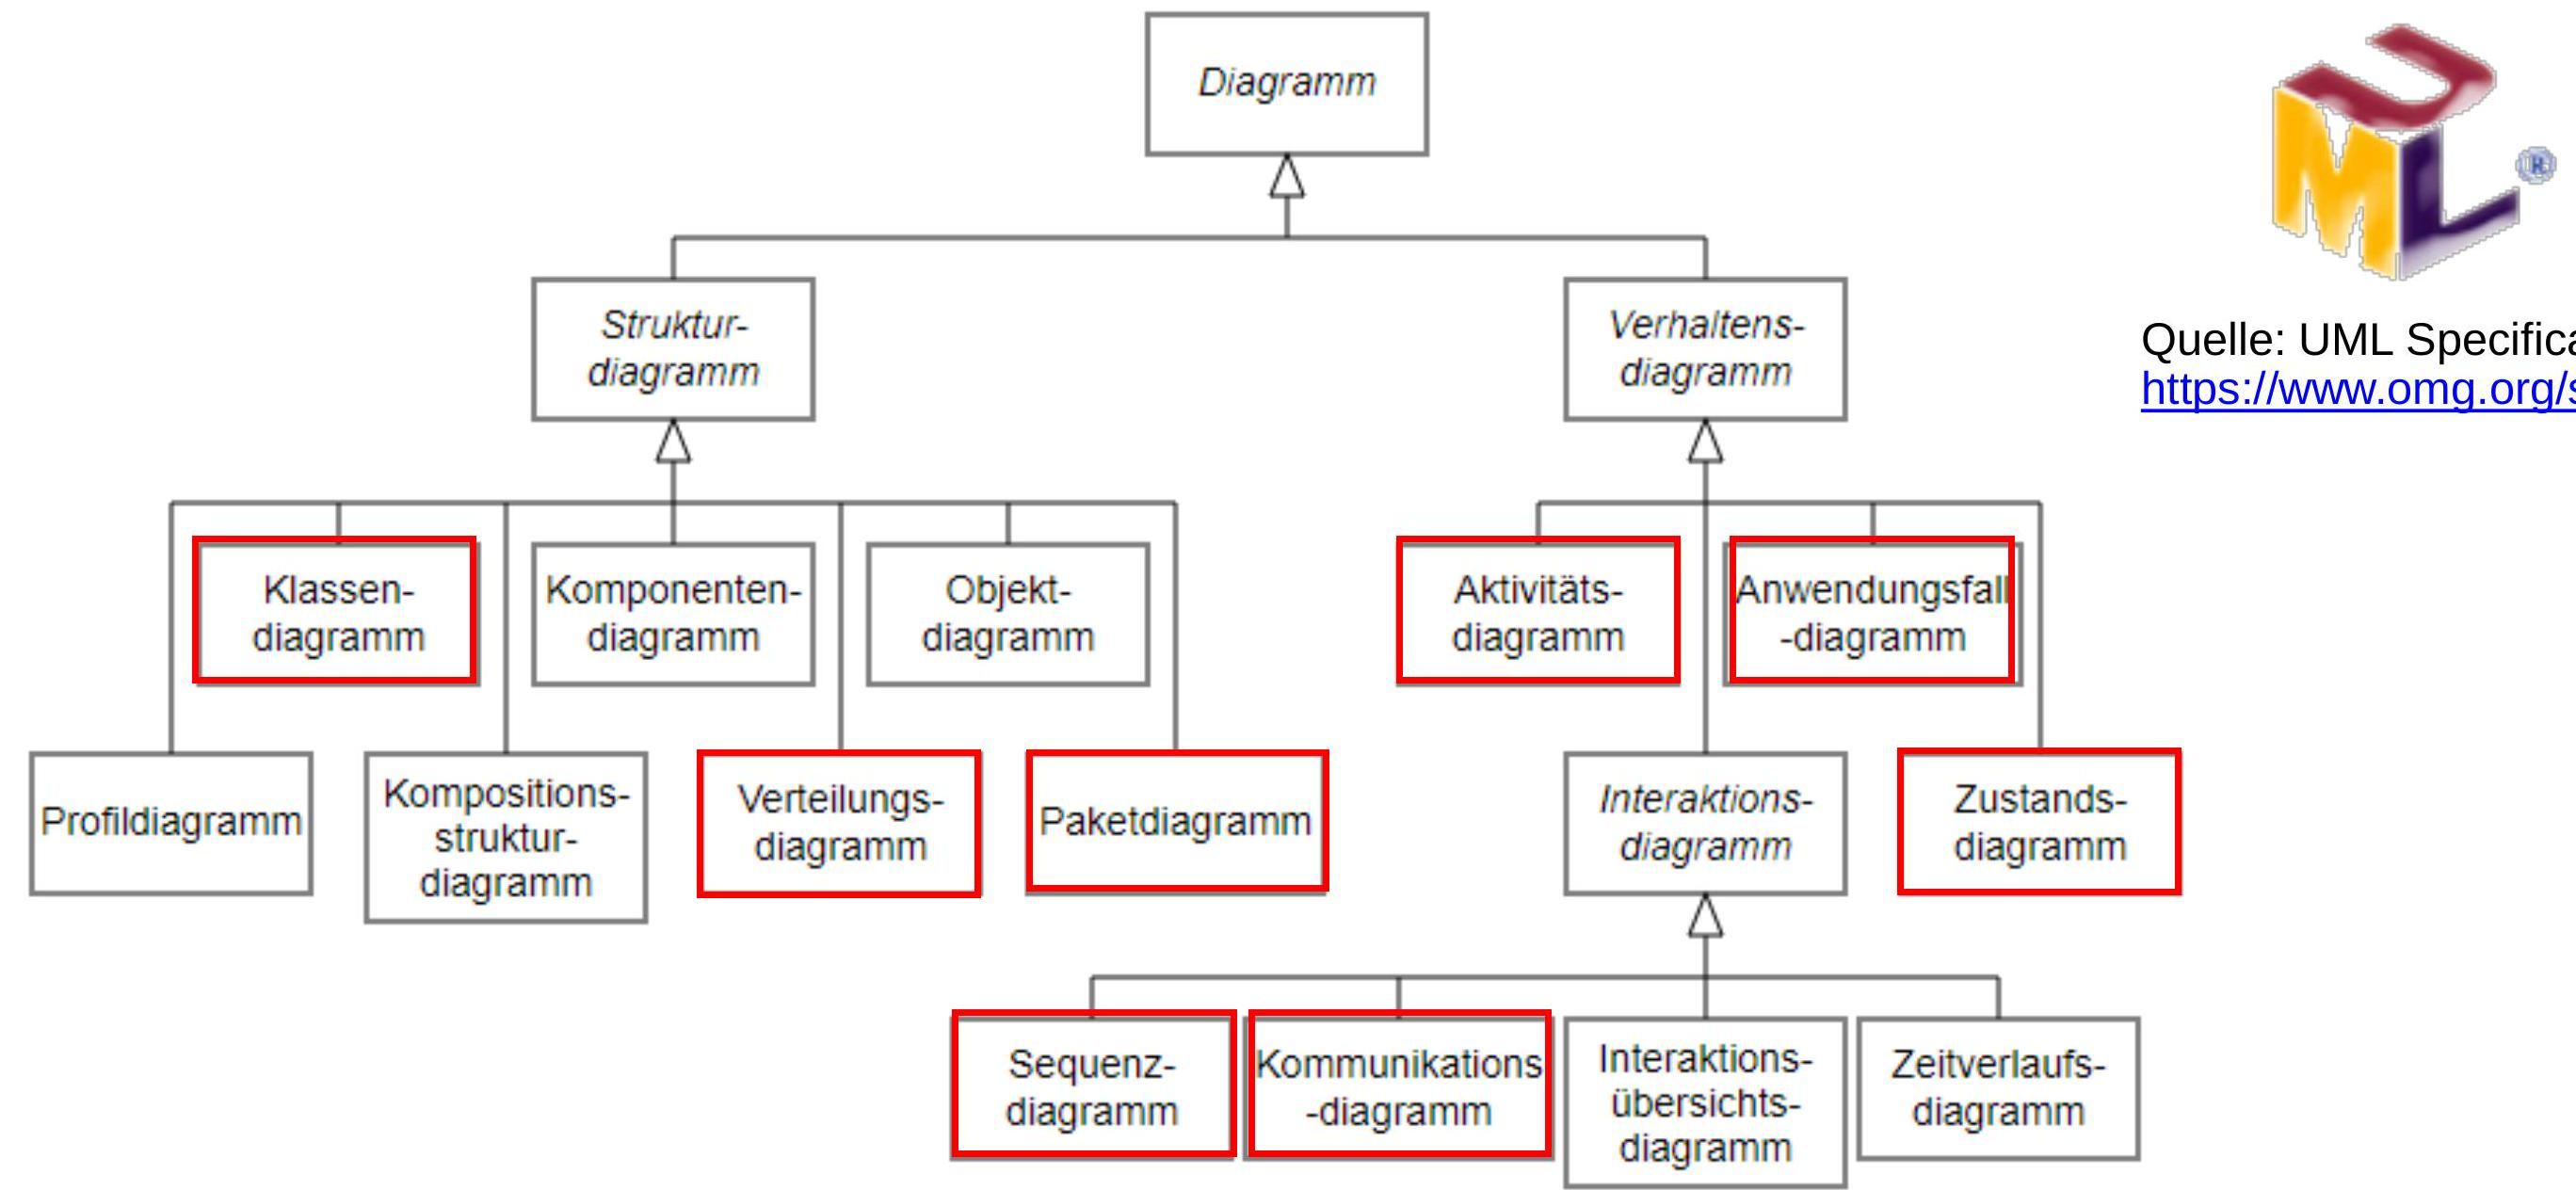
\includegraphics[width=\linewidth]{images/2025_01_02_6eafa38dd4ae10c9a392g-10(1)}

Quelle: UML Specification, \href{https://www.omg.org/spec/UML/}{https://www.omg.org/spec/UML/}\\
$\square$ für die Modellierung in SWEN1 relevant

\section*{Gebrauch der UML (nach Martin Fowler)}
\section*{- UML as a Sketch}
\begin{itemize}
  \item Informelle und unvollständige Diagramme (z.T. von Hand gezeichnet), um schwierige Teile des Problems oder der Lösung zu verstehen und zu kommunizieren
  \item Die agile Community bevorzugt diese Anwendungsart von UML
  \item UML as a Blueprint
  \item Relativ detaillierte Analyse und Design-Diagramme für Code-Generierung oder um existierenden Code besser zu verstehen
  \item Klassische UML-Tools für ein Forward- und Reverse-Engineering (Roundtrip)
  \item UML as a Programming Language
  \item Komplete, ausführbare Spezifikation eines Software-Systems in UML
  \item MDA-Tools zur Modellierung und Generierung
\end{itemize}

\section*{Überblick Anforderungen \& Analyse}
\begin{itemize}
  \item User Research (Personas und Szenarien, Contextual Inquiry)
  \item Sketching und Protoyping
  \item Ableiten und Modellieren von Use Cases (dt. Anwendungsfälle)
  \item Detaillierung der Use Case (UML-Use-Case-Diagramm, Use-CaseSpezifikationen, UI-Sketching
  \item Qualitätsanforderungen und Randbedingungen erheben und festhalten.
  \item Modellierung der Fachlichkeit und Begriffe des Anwenders in einem Domänenmodell (konzeptuelles UML-Klassendiagramm)
  \item Bei der objektorientierten Analyse (OOA) liegt die Betonung darauf, die Objekte - oder Konzepte in dem Problembereich zu finden und zu beschreiben!
\end{itemize}

\section*{Überblick Design}
\begin{itemize}
  \item Design und Modellierung einer für die Problemstellung geeigneten Softwarearchitektur (UML-Paketdiagramm, UML-Verteilungsdiagramm)
  \item Use-Case-Realisierung und Klassendesign mit Verantwortlichkeiten (UML-Klassendiagramm, UML-Sequenzdiagramm, UMLKommunikationsdiagramm, UML-Zustandsdiagramm, UML-\\
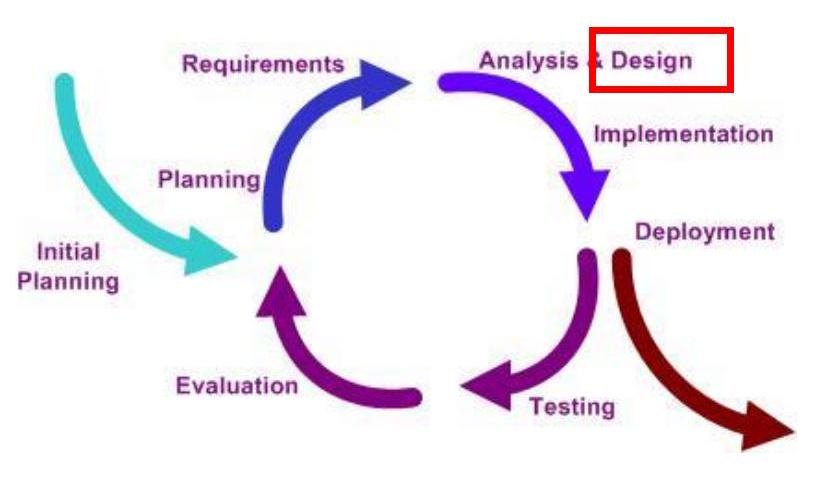
\includegraphics[width=\linewidth]{images/2025_01_02_6eafa38dd4ae10c9a392g-13} Aktivitätsdiagramm)
  \item Entwurf mit bewährten Design Patterns
  \item Beim objektorientierten Design (OOD) liegt die Betonung darauf, geeignete Softwareobjekte und ihr Zusammenwirken (engl. collaboration) zu definieren, um die Anforderungen zu erfüllen!
\end{itemize}

\section*{Überblick Implementation}
\begin{itemize}
  \item Umsetzung des Designs in Code der entsprechenden (objektorientierten) Programmiersprache
  \item Verwendung von geeigneten Algorithmen und Datenstrukturen zur Implementierung des Designs
  \item Code Smells sofort bei deren Aufdeckung verbessern (Refactoring)\\
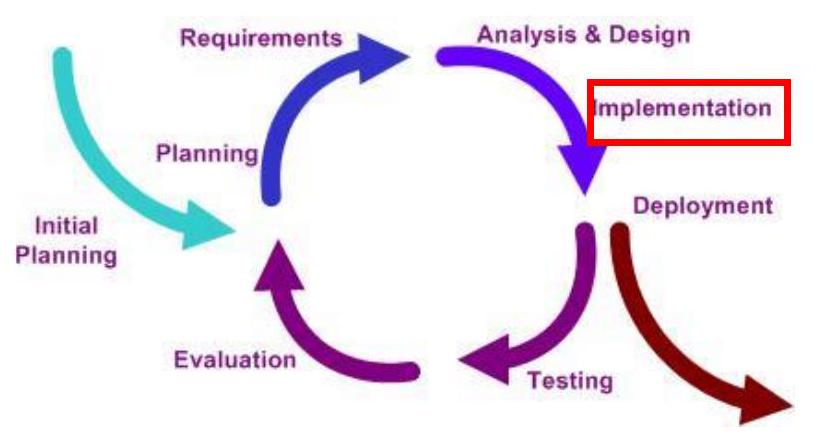
\includegraphics[width=\linewidth]{images/2025_01_02_6eafa38dd4ae10c9a392g-14}
  \item Laufende Dokumentation des Quellcodes (nach Clean CodePrinzipien)
\end{itemize}

\section*{Überblick Testing}
\begin{itemize}
  \item Laufendes Design und Implementierung von Unit-Tests
  \item Planung, Design und Durchführung von weiteren Tests auf den Teststufen Integration und System je nach Problemstellung
  \item Dokumentation des Testkonzepts und der Tests\\
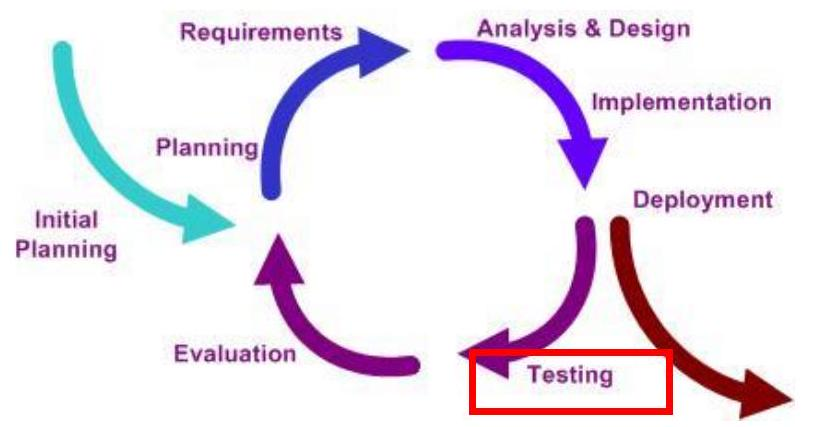
\includegraphics[width=\linewidth]{images/2025_01_02_6eafa38dd4ae10c9a392g-15}
\end{itemize}

\begin{enumerate}
  \item Überblick
  \item Recap Anforderungsanalyse und Domänenmodellierung
  \item Recap Softwarearchitektur und Design
  \item Recap Entwurf mit Design Patterns
  \item Info zur Semesterendprüfung
  \item Bearbeitung einer Fallstudie (alte SEP)
  \item Wrap-up
\end{enumerate}

\section*{Aufgabe 14.1 (10')}
Diskutieren Sie in Murmelgruppen folgende Fragen:

\begin{itemize}
  \item Was ist Usability und wieso ist das wichtig für die Softwareentwicklung?
  \item Wie findet man die wichtigen Anforderungen an ein Softwareprodukt?
  \item Was sind Prozesse und Artefakte in der Anforderungsanalyse für die Softwareentwicklung?
  \item Was ist Domänenmodellierung und was ihr Zweck in der Anforderungsanalyse?
  \item Wieviel Anforderungsanalyse und Domänenmodellierung braucht es für ein Projekt?
\end{itemize}

\section*{Denkpause}
\begin{itemize}
  \item Wieviel Anforderungsanalyse und Domänenmodellierung braucht es für ein Projekt?
  \item Dies hängt von verschiedenen Faktoren eines Software-Projektes ab: Domäne, Grösse (Anzahl MA), Komplexität, Kritikalität, verteilte Entwicklung etc. (s. auch LE 01, Folie 31).
\end{itemize}

\begin{enumerate}
  \item Überblick
  \item Recap Anforderungsanalyse und Domänenmodellierung
  \item Recap Softwarearchitektur und Design
  \item Recap Entwurf mit Design Patterns
  \item Info zur Semesterendprüfung und Q\&A
  \item Bearbeitung einer Fallstudie (alte SEP)
  \item Wrap-up
\end{enumerate}

\section*{Aufgabe 14.2 (10')}
Diskutieren Sie in Murmelgruppen folgende Fragen:

\begin{itemize}
  \item Was ist eine Softwarearchitektur und wie beschreibt man sie?
  \item Was sind die Ziele einer geschichteten Softwarearchitektur und wie beschreibe ich sie?
  \item Wie realisiere ich einen Use Case mit Klassen, die klare Verantwortlichkeiten haben, wartbar und einfach erweiterbar sind?
  \item Wie modelliere ich mein Design (statisches und dynamisches Modell) mit der UML, um es diskutieren und evaluieren zu können?
  \item Wozu sind die GRASP Prinzipien und Patterns im Design nützlich?
\end{itemize}

\begin{enumerate}
  \item Big Picture
  \item Recap Anforderungsanalyse und Domänenmodellierung
  \item Recap Softwarearchitektur und Design
  \item Recap Entwurf mit Design Patterns
  \item Info zur Semesterendprüfung
  \item Bearbeitung einer Fallstudie (alte SEP)
  \item Wrap-up
\end{enumerate}

\section*{Denkpause}
\section*{Aufgabe 14.3 (10')}
Diskutieren Sie in Murmelgruppen folgende Fragen:

\begin{itemize}
  \item Was sind Design Patterns und wozu sind sie nützlich?
  \item Wie wird ein Design Pattern beschrieben?
  \item Welche GoF Design Pattern kennen Sie und was ist ihr Zweck?
  \item Was sind Trade-offs bei der Anwendung eines Design Patterns?
\end{itemize}

\begin{enumerate}
  \item Überblick
  \item Recap Anforderungsanalyse und Domänenmodellierung
  \item Recap Softwarearchitektur und Design
  \item Recap Entwurf mit Design Patterns
  \item Info zur Semesterendprüfung
  \item Bearbeitung einer Fallstudie (alte SEP)
  \item Wrap-up
\end{enumerate}

\begin{itemize}
  \item 2 Quizzes in der Vorlesung während dem Semester zur formativen Lernkontrolle (jeweils 10 Multiple-Choice-Fragen, 15 Min.)
  \item 1 Quiz zur Anforderungsanalyse
  \item 1 Quiz zur Softwarearchitektur und Design
  \item Die erreichte Note zählt zu 10\% für die Gesamtnote
  \item Unterrichtsaufgaben während des Semesters
  \item Max. 3 Punkte pro LE
  \item Die erreichten Punkte zählen zu 20\% für die SEP
  \item Semesterendprüfung (SEP) (90 Min.)
  \item Umfang: Vorlesung, abgegebene Unterlagen, Aufgaben aus dem integrierten Praktikum und der Wissenssicherung
  \item Die erreichte Note zählt zu 90\% für die Gesamtnote
\end{itemize}

\section*{- Inhalte der Semesterendprüfung (SEP)}
\begin{itemize}
  \item 25-35\% Anforderungsanalyse und Domänenmodellierung
  \item 10-20\% Fragen zu Diagrammen und Design mit der UML
  \item 45-65\% Softwarearchitektur und Design, Design Patterns
  \item Umfang ist alles aus den Lerneinheiten 1-9 und zusätzliche GoF Design Patterns aus der Vertiefung V4 (Abstract Factory, Factory Method, Command, Template Method)
  \item Keine Fragen oder Aufgaben zu diskutierter Technologie in den Vertiefungen 1-4 (z.B. zu JavaFX, RMI, REST, WebSocket, JDBC, JPA, Java Reflection etc.)
  \item Inhalte aus den Lernaufgaben und den Wissensicherungen.
\end{itemize}

\begin{enumerate}
  \item Überblick
  \item Recap Anforderungsanalyse und
\end{enumerate}

Domänenmodellierung\\
3. Recap Softwarearchitektur und Design\\
4. Recap Entwurf mit Design Patterns\\
5. Info zur Semesterendprüfung\\
6. Bearbeitung einer Fallstudie (alte SEP)\\
7. Wrap-up

\begin{enumerate}
  \item Überblick
  \item Recap Anforderungsanalyse und\\
Domänenmodellierung
  \item Recap Softwarearchitektur und Design
  \item Recap Entwurf mit Design Patterns
  \item Info zur Semesterendprüfung
  \item Bearbeitung einer Fallstudie (alte SEP)
  \item Wrap-up
\end{enumerate}

\section*{Besprechung Ihres Feedbacks zur Vorlesung}
\begin{itemize}
  \item Gerne nehmen wir noch weiteres Feedback zur Vorlesung entgegen:
  \item Was hat gefallen?
  \item Was hat nicht gefallen?
  \item Was muss geändert werden?
\end{itemize}

Herzlichen Dank und weiterhin viel Erfolg im Studium!


\end{document}